%%
% The BIThesis Template for Bachelor Graduation Thesis
%
% 北京理工大学毕业设计(论文)第二章节 —— 使用 XeLaTeX 编译
%
% Copyright 2020-2023 BITNP
%
% This work may be distributed and/or modified under the
% conditions of the LaTeX Project Public License, either version 1.3
% of this license or (at your option) any later version.
% The latest version of this license is in
%   http://www.latex-project.org/lppl.txt
% and version 1.3 or later is part of all distributions of LaTeX
% version 2005/12/01 or later.
%
% This work has the LPPL maintenance status `maintained'.
%
% The Current Maintainer of this work is Feng Kaiyu.
%%

\chapter{相关理论}
{本章将介绍本文相关的理论知识和一些计算方法,以了解心动运动规律和心脏特征提取处理的方法。}
\section{心血管系统动力学}
{心脏通过交替的心肌收缩和放松将血液泵入血管,从而形成一种周期性的心跳模式,称为心动周期。而血液通过心血管系统送到全身,包括指尖。人体心脏包含四个心室(即左上心房和 右上心房;左下心室和右下心室)。心动周期一般指从一次心跳的起始到下一次心跳的起始心血管系统所经历的过程\cite{2006The},典型的心动周期通常包括八个周期:等容收缩期、快速射血期、等容舒张期、心房收缩期:}
\par
\begin{figure}[htbp]
  \centering
  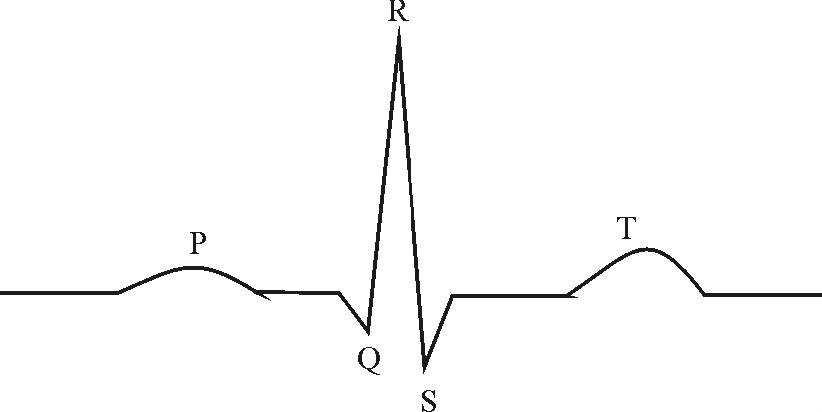
\includegraphics[width=0.5\linewidth]{images/R.png}
  \caption{一个正常心动周期\cite{2018sun}}\label{2-1} % label 用来在文中索引
\end{figure}
\par
\begin{itemize}
\item {\bf{等容收缩期}:} {心室开始收缩,对应心电图R波顶峰时刻,如图2-1所示。心室肌的强有力的收缩使心室内压急剧升高。当超过心房内压时,左右心室内血液即分别推动左右房室瓣使其关闭。由于乳头肌与腱索拉紧房室瓣,阻止其向上翻入心房,再加房室交界处环行肌收缩,缩小房室交界处的口径,两者都可避免心室血液倒流心房。这时室内压急剧上升,但在未超过主动脉压(舒张期末约为80毫米汞柱)和肺动脉压(舒张期末约为8$\sim$10毫米汞柱)时,半月瓣仍处于关闭状态。在这段短时间内(在人体平均为0.05秒),房室瓣与半月瓣均关闭,心尖到基底部的长度减小,心室变得较圆,心室肌张力增高,而心室容积不变,故称等容收缩期。}
\item {\bf{快速射血期}:} {心室肌继续收缩,张力增高,心室内压急剧上升,很快超过主动脉压和肺动脉压,两侧半月瓣被冲开,血液射入主动脉和肺动脉并很快达到最大速率。快速射血期末心室压力达到顶峰(左心室约120$\sim$130毫米汞柱,右心室约24$\sim$25毫米汞柱)。此期平均历时0.09秒,约占心缩期的1/3时间,而射出的血量占每搏输出量的80$\sim$85$\%$。 }
\item {\bf{等容舒张期}:} {心室开始舒张,射血停止,心室内压急速下降。左心室压原已略低于主动脉压,而右心室压迅速降到低于肺动脉压,此时两侧半月瓣迅速关闭,阻止血液倒流入心室。从心室舒张开始到半月瓣关闭这一段时间,称为舒张前期,历时约0.04秒。}
\item {\bf{心房收缩期}:} {在心室舒张期末,心房开始收缩,心房内压升高将残留的血液射入心室,使心室充盈度进一步提高,心室压力也出现一个小的升高。心房的舒张使房内压降低,这有助于房室瓣的关闭,故在心室收缩前房室瓣已有关闭的趋势。至下一次等容收缩开始时,即完成一个心动周期。}
\end{itemize}

{脏舒张时内压降低,腔静脉血液回流入心,心脏收缩时内压升高,将血液泵到动脉。心脏每收缩和舒张一次构成一个心动周期。一个心动周期中首先是两心房收缩,其中右心房的收缩略先于左心房。心房开始舒张后两心室收缩,而左心室的收缩略先于右心室。在心室舒张的后期心房又开始收缩。如以成年人平均心率每分钟75次计,每一心动周期平均为0.8秒,其中心房收缩期平均为0.11秒,舒张期平均为0.69秒。心室收缩期平均为0.27秒,舒张期平均为0.53秒\cite{2006The}。}
\par
{本文的心动周期划分是使用手机摄像头采集视频,使用视频帧图像的像素点的红色通道平均光强为参考数据,寻找视频流时间序列的波谷进行划分,划分心动周期一般由心室射血开始,经历心室射血、等容舒张、心房收缩和等容收缩四个阶段。}


\section{摄像头捕捉心脏运动}
{
由于心脏运动模式固有且唯一,每个人的心跳运动具有独特性,因此,工作重点是有效地提取心跳生物特征。与依赖现有的专用的心脏运动特征捕捉器不同,本文寻求通过现有的商用设备来检测并反应指尖血液流动,以获取用户的心脏运动特征。通过智能手机的内置摄像头捕获人体指尖皮肤的反射光来观察连续血流引起的光吸收变化,其中包含了独特的心脏运动特征\cite{2007Photoplethysmography}。
}
\par
{
总的来说,内置摄像头的每个像素充当独立的光线传感器,以检测指尖上的光线变化。由于当前智能手机摄像头分辨率高(例如每帧1280×720像素),因此可以实现精细的心动周期监测。另外,每个像素的三个颜色通道(红、蓝、绿)为有效的特征提取提供了多个维度。每个像素点支持红、绿、蓝三个颜色通道,因此内置摄像头除了能捕捉心脏特征用于心脏动态检测之外\cite{2007Photoplethysmography},还能反应人的皮肤反特征。
}
\begin{figure}[htp]
\centering
    \begin{minipage}[t]{0.49\textwidth}
        \centering
        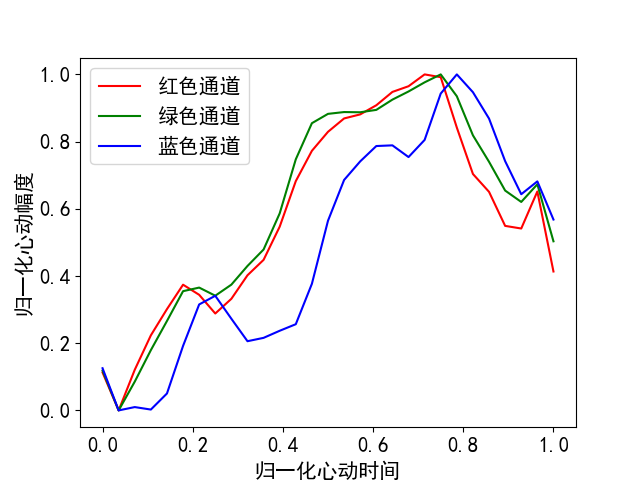
\includegraphics[width=1\textwidth]{images/Figure_8.png}
        \caption{志愿者1归一化三色通道光强图}
        \label{2-2}
    \end{minipage}
    \begin{minipage}[t]{0.49\textwidth}
        \centering
        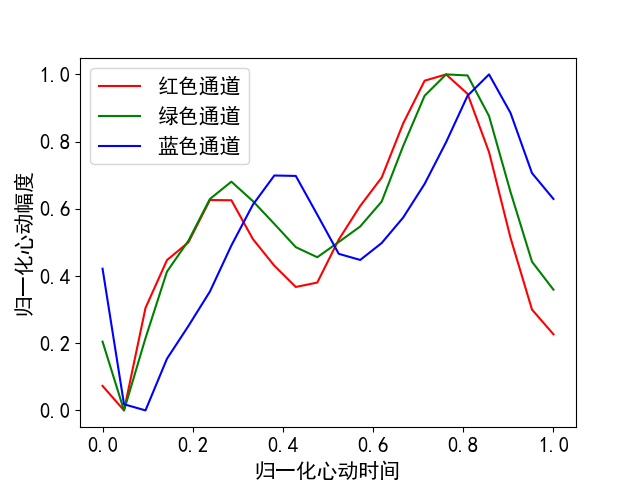
\includegraphics[width=1\textwidth]{images/Figure_9.png}
        \caption{志愿者2归一化三色通道光强图}
        \label{2-3}
        \end{minipage}
\end{figure}
\par
{图2-1和图2-2为不同用户通过手机摄像头获取的单个周期内三色通道的光强度变化,并归一化以消除心率不同带来的影响,很明显两名测试者在单个心动周期内的心脏运动模式在三个颜色通道内均不同,同一用户的心脏运动模式在不同颜色通道上体现出的特征也不同,者为特征提取提供了冗余特征。}

\section{巴特沃斯数字滤波器}
{巴特沃斯数字滤波器是IIR 数字滤波器的一种,由于其频率响应在通频带内具有最大限度平坦,因此对音频信号的平滑处理具有较好的效果,是一种应用较为广泛的滤波器\cite{2012zhang}。}
\par
{巴特沃斯滤波器的特点是通频带的频率响应曲线最平滑\cite{2006wang},即之前欺负较大的曲线在滤波后的频率响应曲线在通过的频率带范围内十分平滑,几乎没有起伏,而被阻止的频率带则下降到零。使用巴特沃斯低通滤波器处理信号不仅可以过滤掉干扰频段的信号,还可以排除由于手指颤抖导致心波信号大幅度起伏变化,对低频段的音频信号进行平滑处理有较好的效果\cite{2012zhang}。}
\par
{实现示例:}
\begin{algorithm}
        \caption{巴特沃斯数字滤波器}
        \begin{algorithmic}[1] %每行显示行号
        \Require $data$是需要滤波的数据,$h$是滤波结果
            \State $W_p=0.2*pi;W_s=0.3*pi$ \hspace{7em}{\#设置通带上限频率和下限频率}
            \State $A_p=1;A_s=60$\hspace{12em}\space{\#设置通带波纹和阻带最小衰减}
            \State $[N,wn]= buttord(Wp/pi,Ws/pi,Ap,As);$\hspace{1em}{\#生成阶数和归一化截至频率}
            \State $[b,a]= butter(N,wn,'bandpass');$\hspace{4em}\space\space\space{\#生成滤波器的分子分母系数向量}
            \State$ h = freqz(b,a,w);$
            
        \end{algorithmic}
    \end{algorithm}
\par
{一阶巴特沃斯滤波器的衰减率为每倍频6分贝,每十倍频20分贝。二阶巴特沃斯滤波器的衰减率为每倍频12分贝,三阶巴特沃斯滤波器的衰减率为每倍频18分贝,如此类推。巴特沃斯滤波器的振幅对角频率单调下降,并且也是唯一的无论阶数、振幅对角频率曲线都保持同样的形状的滤波器。只不过滤波器阶数越高,在阻频带振幅衰减速度越快。其他滤波器高阶的振幅对角频率图和低级数的振幅对角频率有不同的形状。}
\par
{当然巴特沃斯滤波器也存在一些缺点,巴特沃斯滤波器是滤波器的一种设计分类,类同于切比雪夫滤波器,它有高通,低通,带通,带阻等多种滤波器。它在通频带内外都有平稳的幅频特性,但有较长的过渡带,在过渡带上很容易造成失真,在调用巴特沃斯滤波器做仿真时,信号总会在第一个周期略微有些失真。但往后的幅频特性就非常的好。}
\section{主成分分析(PCA)与奇异值分解(SVD)}
\subsection{PCA转换}
{主成分分析(PCA)的主要目标是将特征维度变小,同时尽量减少信息损失。就是对一个样本矩阵,一是换特征,找一组新的特征来重新表示;二是减少特征,新特征的数目要远小于原特征的数目。}
\par
{通过主成分分析(PCA)将n维原始特征映射到维(k<n)上,称这k维特征为主成分。需要强调的是,不是简单地从n 维特征中去除其余n- k维特征,而是重新构造出全新的k维正交特征,且新生成的k维数据尽可能多地包含原来n维数据的信息。例如,使用主成分分析(PCA)将20个相关的特征转化为5个无关的新特征,并且尽可能保留原始数据集的信息。将主成分分析(PCA)转换用于心波特征提取时,可以将原有的特征更多得包含在新的特征空间中,同时在新的特征空间中筛选出影响较大,特征明显的新特征,从而过滤掉一些冗余无用的特征,减轻计算负担。}
\par
{\bf{PCA转换主要涉及几个问题}:}
\begin{itemize}
    \item {对实对称方阵,可以正交对角化,分解为特征向量和特征值,不同特征值对应的特征向量之间止交,即线性无关。特征值表示对应的特征向量的重要程度,特征值越大,代表包含的信息量越多,特征值越小,说明其信息量越少。在等式$Av=\lambda v$中$v$为特征向量,$\lambda$为特征值。}
    \item {方差相当于特征的辨识度,其值越大越好。方差很小,则意味着该特征的取值大部分相同,即该特征不带有效信息,没有区分度;方差很大,则意味着该特征带有大量信息,有区分度。因此在降维后通常选择方差较大的主分析成分。}
    \item {协方差表示不同特征之间的相关程序,例如,考察特征$x$和$y$的协方差,如果是正值,则表明$x$和$y$正相关,即$x$和$y$的变化趋势相同,越大$y$越大;如果是负值,则表明$x$和$y$负相关,即$x$和$y$的变化趋势相反,$x$越小$y$越大;如果是零,则表明$x$和$y$没有关系,是相互独立的。在心波特征提取过程中,特性之间的独立性越强,说明特征提取效果越好。}
\end{itemize}
\par
{\bf{PCA求解步骤}:}
\par
{首先我们输入$m$条样本,特征数为$n$的数据集,即样本数据$X=[x_1,x_2,\dots ,X_m]$,降维到的目标维数为k。记样本集为矩阵$X$。}
\begin{equation}
    X=\begin{bmatrix}
        X_{11} & X{12} & \dots & X_{1n} \\
        X_{21} & X{22} & \dots & X_{2n} \\
        \dots  & \dots  & \dots & \dots  \\
        X_{m1} & X{m2} & \dots & X_{mn} 
    \end{bmatrix}
\end{equation}

\par
{其中每一行代表一个样本,每一列代表一个特征,列号表示特征的维度,共$n$维。}
\begin{itemize}
    \item {第一步,对矩阵去中心化得到新矩阵$X$,即每一列进行零均值化,也即减去这一列的均值$\overline{x_i}$,$\overline{x_i}=\frac{1}{m}\sum_{j=1}^{m}{X_{ji}},(i=1,2,3,\dots ,n)$所求$X$仍为$m\times n$阶矩阵。}
    \begin{equation}
    X=\begin{bmatrix}
        X_{11}-\overline{x_1} & X{12}-\overline{x_2} & \dots & X_{1n}-\overline{x_n} \\
        X_{21}-\overline{x_1} & X{22}-\overline{x_2} & \dots & X_{2n}-\overline{x_n} \\
        \dots  & \dots  & \dots & \dots  \\
        X_{m1}-\overline{x_1} & X{m2}-\overline{x_2} & \dots & X_{mn}-\overline{x_n} 
    \end{bmatrix}
\end{equation}
    \item {第二步,计算去中心化的矩阵$X$的协方差矩阵$C=\frac{1}{m-1}{X^{T}X}$,即$n\times n$阶矩阵。}
    \item {第三步,对协方差矩阵$C$进行特征分解,求出协方差矩阵的特征值$\lambda_k$,及对应的特征向量$v_k$,即$Cv_k=\lambda_kv_k$。}
    \item {第四步,将特征向量按对应特征值从左到右按列降序排列成矩阵,取前$k$列组成矩阵$W$,即$n\times k$阶矩阵。}
    \item {第五步,通过$Y=XW$计算降维到$k$维后的样本特征,即$m\times K$阶矩阵。}
\end{itemize}
\par
{由上述步骤得到的矩阵$Y$就是降维到$k$维后的新样本集,其中每一行代表一个样本,每一列代表一个特征,特征由原来的$n$维降低到了$k维$。其中第四五步可以调换顺序,先进行特征变换之后再挑选k个主分析成分。}
\subsection{奇异值分解(SVD)}
{
由于非$N\times N$的满秩矩阵无法进行特征分解,为了解决这一问题,奇异值分解(SVD)被提出\cite{ 1993Singular},它可以很容易得到任意矩阵的满秩分解,用满秩分解可以对数据做压缩,并且可以把矩阵和空间关系对应起来\cite{1996A}。对于任意矩阵都可以做到如下分解:
}
\begin{equation}
    A_{m\times n}=U_{m\times m}\times S_{m\times n}\times V_{n\times n}
\end{equation}
\begin{figure}[htbp]
  \centering
  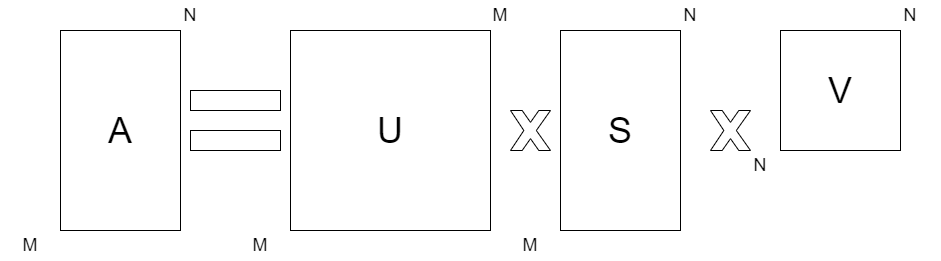
\includegraphics[width=1.0\linewidth]{images/svd.drawio.png}
  \caption{SVD分解示意图}\label{2-4} % label 用来在文中索引
\end{figure}
\par
{SVD分解步骤如下:}
\begin{itemize}
    \item {第一步将矩阵$AA^{T}$进行特征分解,获得$m$个特征值$\lambda_i$和对应的特征向量$v_i$,根据特征值的大小从大道小排列,对应的特征向量作为列向量组成矩阵$U=[v_1,v_2,\dots,v_m]$,其中$\lambda_1>\lambda_2>\dots >\lambda_m$。}
    \item {第二步将矩阵$A^{T}A$进行特征分解,获得$n$特征值$\lambda_i$和对应的特征向量$v_i$,根据特征值的大小从大道小排列,对应的特征向量作为行向量组成矩阵$V^{T}=[v_1,v_2,\dots,v_n]$,其中$\lambda_1>\lambda_2>\dots >\lambda_n$。}
    \item {第三步根据矩阵$A^{T}A$求出的特征值$\lambda_1,\lambda_2,\dots,\lambda_n$,求出$n$个奇异值$\sigma_i$,其中$\sigma_i=\sqrt{\lambda_i},i=1,2,\dots,n$,奇异值$\sigma_i$对角排列即为矩阵$S$。}
\end{itemize}
\par
{如图2-4所示,SVD分解可以将任意矩阵进行分解,中间的矩阵S是奇异值矩阵,除了对角线上是奇异值外其他都是零。}
\subsection{使用奇异值分解(SVD)实现PCA转换}
{PCA转换的实质就是求一个矩阵$W$使得$Y=XW$所得的矩阵$Y$从从原来的向量空间映射道特性无关的新空间,PCA转换与SVD分解都有相同的操作,即对矩阵$AA^{T}$进行特征分解,因此可以使用SVD分解出的矩阵$U$进行PCA特征转换。吴春国、梁艳春等人对PCA和SVD等价性进行了研究\cite{2004wu},在前人的基础上证明SVD分解与PCA转换具有等价性。利用SVD分解对提取的心脏特征进行PCA转换将简化计算过程,降低系统复杂度。}